\section{Results}
\label{sec:results}

By estimating the time series of COVID-19 infections per 100,000 inhabitants
for each \US state from June 1, 2020 to November 29, 2021, we observe rates of
infections that vary in intensity and disease burden across space and time
(Figures \ref{fig:state_infect_est}--\ref{fig:six-states}). Outbreaks in
infections precede those in cases and are consistently larger in magnitude
(we will often take ``cases'' to mean ``reported cases'').

The largest per-capita outbreaks prior to Omicron were observed in the late
summer or early fall of 2021 in Louisiana, Georgia, Idaho, and Montana
matching the intuition of similar viral spread in clusters of geographically
proximate states. During this time, the two states that have the highest rate of
infections on single day are Louisiana (476 infections per 100K, on July 20, 2021,
2021) and Idaho (also 457 infections per 100K, on September 7, 2021). The period
of lowest viral transmission is observed in the summer of 2020. From June 2020
to the end of August, Vermont saw less than 10 infections per 100K per week,
the longest such lull for any state.



\subsection{Infection estimates reveal waves missed by reported cases}
\label{sec:omitted-waves}

Relative to reported cases, examining estimated infections reveals a
rather different pattern. \autoref{fig:state_infect_est} shows
estimates of the number of daily new infections per 100,000 inhabitants for each
\US state from June 1, 2020 to November 29, 2021 compared with reported cases,
and deconvolved cases---reported cases ``pushed back'' by the delays shown in
\autoref{fig:chain_events_onset_report}. 

Nearly all states exhibit at least two major spikes in infections---the first starts
in the fall of 2020 and extends into the winter season, while the second starts
in the late summer of 2021 and proceeds into the mid-fall. These represent major
waves driven by the Ancestral and Delta variants, respectively. 
In general, greater similarities in the strength and magnitude of
outbreaks emerge in small clusters of states that border each other.
For instance, in the Western states of Idaho and Montana 
or in the Southern states of North and South Carolina 
the crests and troughs in the waves of infections appear to mirror each other.
Compared to the other states, consistently low rates of infections are attained in the
Northeastern states of Vermont, New Hampshire, and Maine, even during
the aforementioned Ancestral and Delta waves.

While the major Ancestral, Alpha, and Delta waves tend to be visible for most
states, there are clear outbreaks in unreported infections that are not easily
detectable from cases alone in the falls of 2020 and 2021. For example, a wave 
of infections is evident in North Dakota and South Dakota over the spring of 2021
that is virtually undetectable from the reported cases. In the late summer of 2021, the
Delta wave is only faintly detectable from cases in a number of Northeastern
states (New York, Massachusetts, Connecticut, and New Hampshire), and yet
the infections suggest that it has already begun in earnest. 

\subsection{The cases-to-infections ratio varies by state and variant}
\label{sec:case-infection-ratio}

\begin{figure}[!tb]
\centering
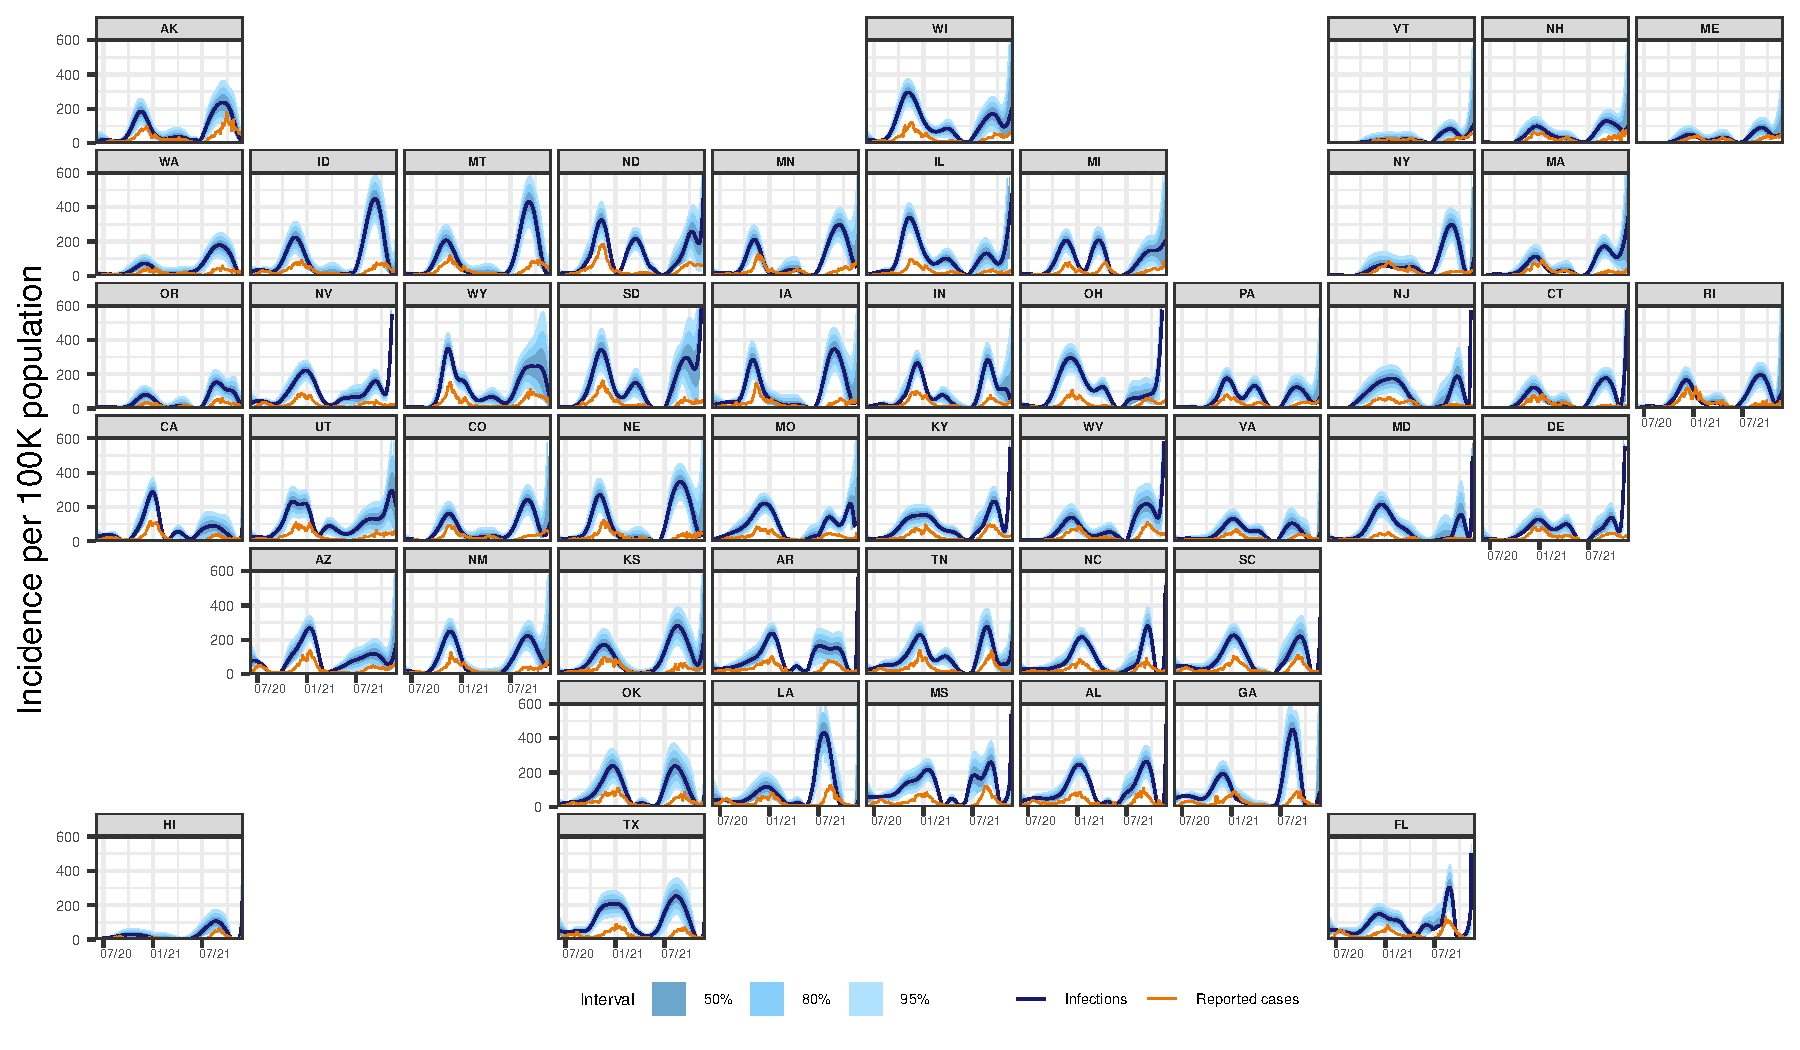
\includegraphics[width=.99\linewidth]{adj-unadj-cases-plot-1.pdf} 
\caption{Estimates of the number of daily new infections per 100,000
population for each \US state from June 1, 2020 to November 29, 2021
(dark blue line). The blue shaded regions depict the 50, 80, and 95\%
intervals for the estimates, while the teal line represents
the number of new daily new deconvolved cases per 100,000, and the
orange line represents the trailing 7-day average of reported cases per
100,000.}
\label{fig:state_infect_est}
\end{figure}    

While it is clear from \autoref{fig:state_infect_est} that cases underestimate
the true burden of infections for every state, the degree to which this problem
persists varies across states and variants. 
For the Ancestral wave, the largest
discrepancies are more frequently in the Midwest: states such as Illinois,
Indiana, and Ohio. 
For the Delta wave, some of the
largest discrepancies between cases and infections are visible in the Western
states of Idaho and Montana, the Southern states of Louisiana and Georgia, and
the Midwestern states of Iowa and Nebraska. 
Early in the pandemic, such discrepancies between cases and
infections may be attributable to state-specific issues with the reporting
pipeline, while later, they more likely due to the rise in asymptomatic
infections across variants \citep{oph2022covid, garrett2022high}. 

The ratio between cases and infections decreases with time. While the Delta wave
is somewhat apparent from the case counts for all states
(\autoref{fig:state_infect_est}), infection estimates suggest that case counts
severely underestimate infections during this time for many states, more so than
in earlier waves. The most extreme was New Jersey, where about 6.3\% of
estimated infections were eventually reported as cases. Similarly low are
Maryland (7.3\%), and Nevada (8.4\%), and South Dakota (10.0\%). This issue extends
to most states: in 44 states fewer than 30\% of infections eventually appear in
case reports. This ratio was less extreme in earlier waves, and its effects most
apparent in different regions. During Alpha, Louisiana had the lowest ratio of
infections to cases (11.9\%) followed by California (13.6\%). Such patterns are
less apparent during the Ancestral wave, where Ohio and Maryland had the
lowest ratio of reported cases to infections at 21.4\% and 21.7\%,
respectively. 

\autoref{fig:choro_inf_case_rates} displays the
state-level daily new infections and cases per 100,000 for five dates over
June 2020 to November 2021, 
allowing a closer examination of the spatial trends for these dates.
For instance, it shows that on June 1, 2020, there is little
difference between case and infection rates across the states, while later on,
the differences become more pronounced. It also shows that 
using cases as a proxy for infections can lead to misunderstandings in the 
states that are affected and the extent of that each are affected.
For some days, the spatial extent of infections is understated by
cases. For example, on October 20, 2020, while case rates are elevated in a
handful of upper-Midwestern states (namely, North and South Dakota), infection
estimates are elevated to a similar extend in the surrounding states, emphasizing a
wider impact than is indicated by cases. On July 20, 2021, while the
map of case rates shows low and geographically consistent spread, infection
rates reveal that Texas, Louisiana, Georgia, and their neighbors are hotspots at
that time. 

By focusing on states with elevated cases, infection outbreaks may be
overlooked. For instance, on August 27, 2021, Montana and Idaho have some of the
highest infection rates. In contrast, the case rates are unremarkable for these
two states, whereas the highest rates tend to be localized to the Southeastern
states. However, the opposite occurs as well: on December
17, 2020, Tennessee and California have the highest case rates but comparatively
similar  infections relative to other states.

\begin{figure}[!tb]
\centering
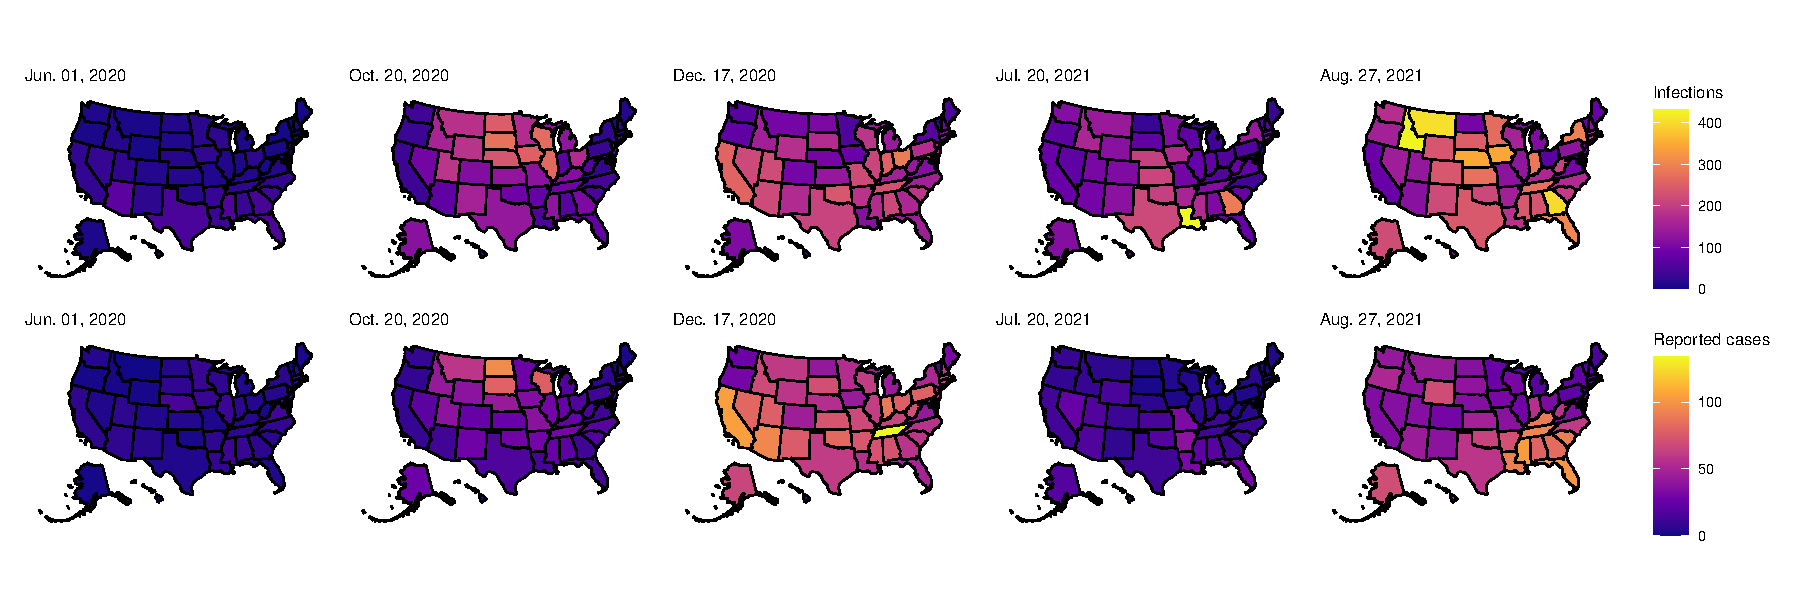
\includegraphics[width=.99\textwidth]{choro-maps-1.pdf}
\caption{Choropleth maps of the state-level estimates of the number of daily new
infections per $100,000$ population (top row) and the daily new cases per
$100,000$ population (bottom row) for five dates between June 1, 2020 and
November 29, 2021. Note that the first date was chosen as a baseline, while the
other dates were chosen due because they show large counts of infections across all
states. In particular, the third and fifth dates present the largest number of
total infections across the 50 states within those calendar years.} 
\label{fig:choro_inf_case_rates}
\end{figure}    



    
\subsection{Infections, overall and by variant, emphasize earlier outbreaks}
\label{sec:infections-by-voc}

\autoref{fig:six-states} examines the infection estimates for a selection of
states more closely. The top panel shows infection estimates for these states,
while the bottom panel disaggregates their deconvolved cases based on the locally
circulating variant proportions at the time. These figures show times when the
total infections and the deconvolved cases by variant emphasize earlier
outbreaks than are indicated by cases alone. During the Ancestral
wave, infections in Massachusetts, Idaho, Montana, Louisiana, and Ohio peak earlier
than cases. For these states, the infections peak about 17 days
earlier on average, with Massachusetts attaining the maximum difference of 26 days.
Such trends are also observed in the 
major Delta wave in the states that present a prominent peak during this time
such as Montana and Louisiana,
where infections lead cases by about 41 and 24 days, respectively.
The division by variant categories reveals the variant(s) that are behind these waves. For
example, in California alone, a spike in Epsilon appears to occur 
alongside the major spike in Ancestral. To give another example, 
we can see a major increase in Alpha in Massachusetts over the spring
of 2021. To a lesser extent, this trend is apparent for all of the other states,
save for California, where Alpha is not a major driver of infections in
comparison to the other variants in circulation around that time. 

\begin{figure}[!tb]
\centering
    \includegraphics*[width=\linewidth]{six-decon-var-1.pdf}
    \caption{Panel A: Reported cases, deconvolved cases, and estimates of
    daily new infections (dark blue line) per 100K inhabitants. The blue shaded
    regions indicate 50, 80, and 95\% confidence bands.  
    Panel B: Deconvolved cases colored by variant per 100K inhabitants.}
    \label{fig:six-states}
\end{figure}


\subsection{Infections lead hospitalizations according to cross-correlations}
\label{sec:lagged-correlations}

We systematically investigate the temporal relationship between infections and
hospitalizations with Spearman's rank-correlation across different lags
(\autoref{fig:correlations}). The maximum average correlation across states is
0.48, occurring at a lag of 13 days. In contrast, we find that the greatest
average Spearman correlation for cases is 0.69 and occurs at a lag of 1 day.
That is, case reports are nearly contemporaneous to hospitalizations, while
infection estimates clearly precede them. 

With respect to previous literature, 
the maximum correlation being attained at a lag of 13 days is fairly consistent with
with estimates of the average time from infection to
hospitalization for cases reported in January, 2020 in Wuhan, China (9.7 days)
as well as with estimates from across the pandemic in the UK (ranging from 8.0
to 9.7 days) \citep{linton2020incubation, ward2021understanding}. 
Importantly, our 13 day lag for the
\US\ also includes the impact of the reporting pipeline, a delay omitted from
the international estimates. 

\begin{figure}[!tb]
\centering
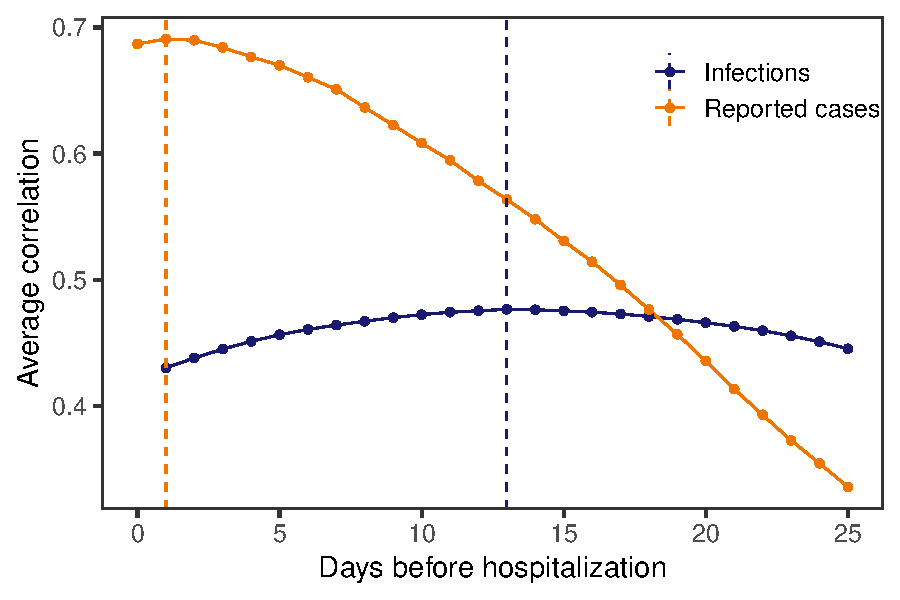
\includegraphics[width=.8\linewidth]{corr-plot-1.pdf} 
\caption{Spearman's correlation between each of cases, deconvolved cases, and
infections with hospitalizations per 100,000. These are calculated for each lag,
state and rolling window of 61 days before averaging. The vertical dashed lines
indicate the lags for which the highest average correlation is attained.}
\label{fig:correlations}
\end{figure}
    

The average correlation is consistently larger for cases than infections 
(with a difference of about 0.21 at the peaks). 
This increase for cases is likely due to two reasons. First, many cases are
detected contemporaneously with hospitalization: people may first test
positive only when they go to to the hospital for treatment. Second, unreported
infections tend to be less severe and less likely to lead to hospitalization
than those that are reported \citep{sallahi2021using}.



\subsection{IHR estimates tend to be smaller and exhibit less pronounced spikes}
\label{sec:ihrs}

As a counterpart to the correlation analysis, we compute the time-varying
infection-hospitalization ratios (IHRs) for each state using the correlation
maximizing lag. We similarly compute the case-hospitalization ratios (CHRs)
using their correlation maximizing lag for comparison
(\autoref{fig:IHR_7dav}). 

\begin{figure}[!tb]
\centering
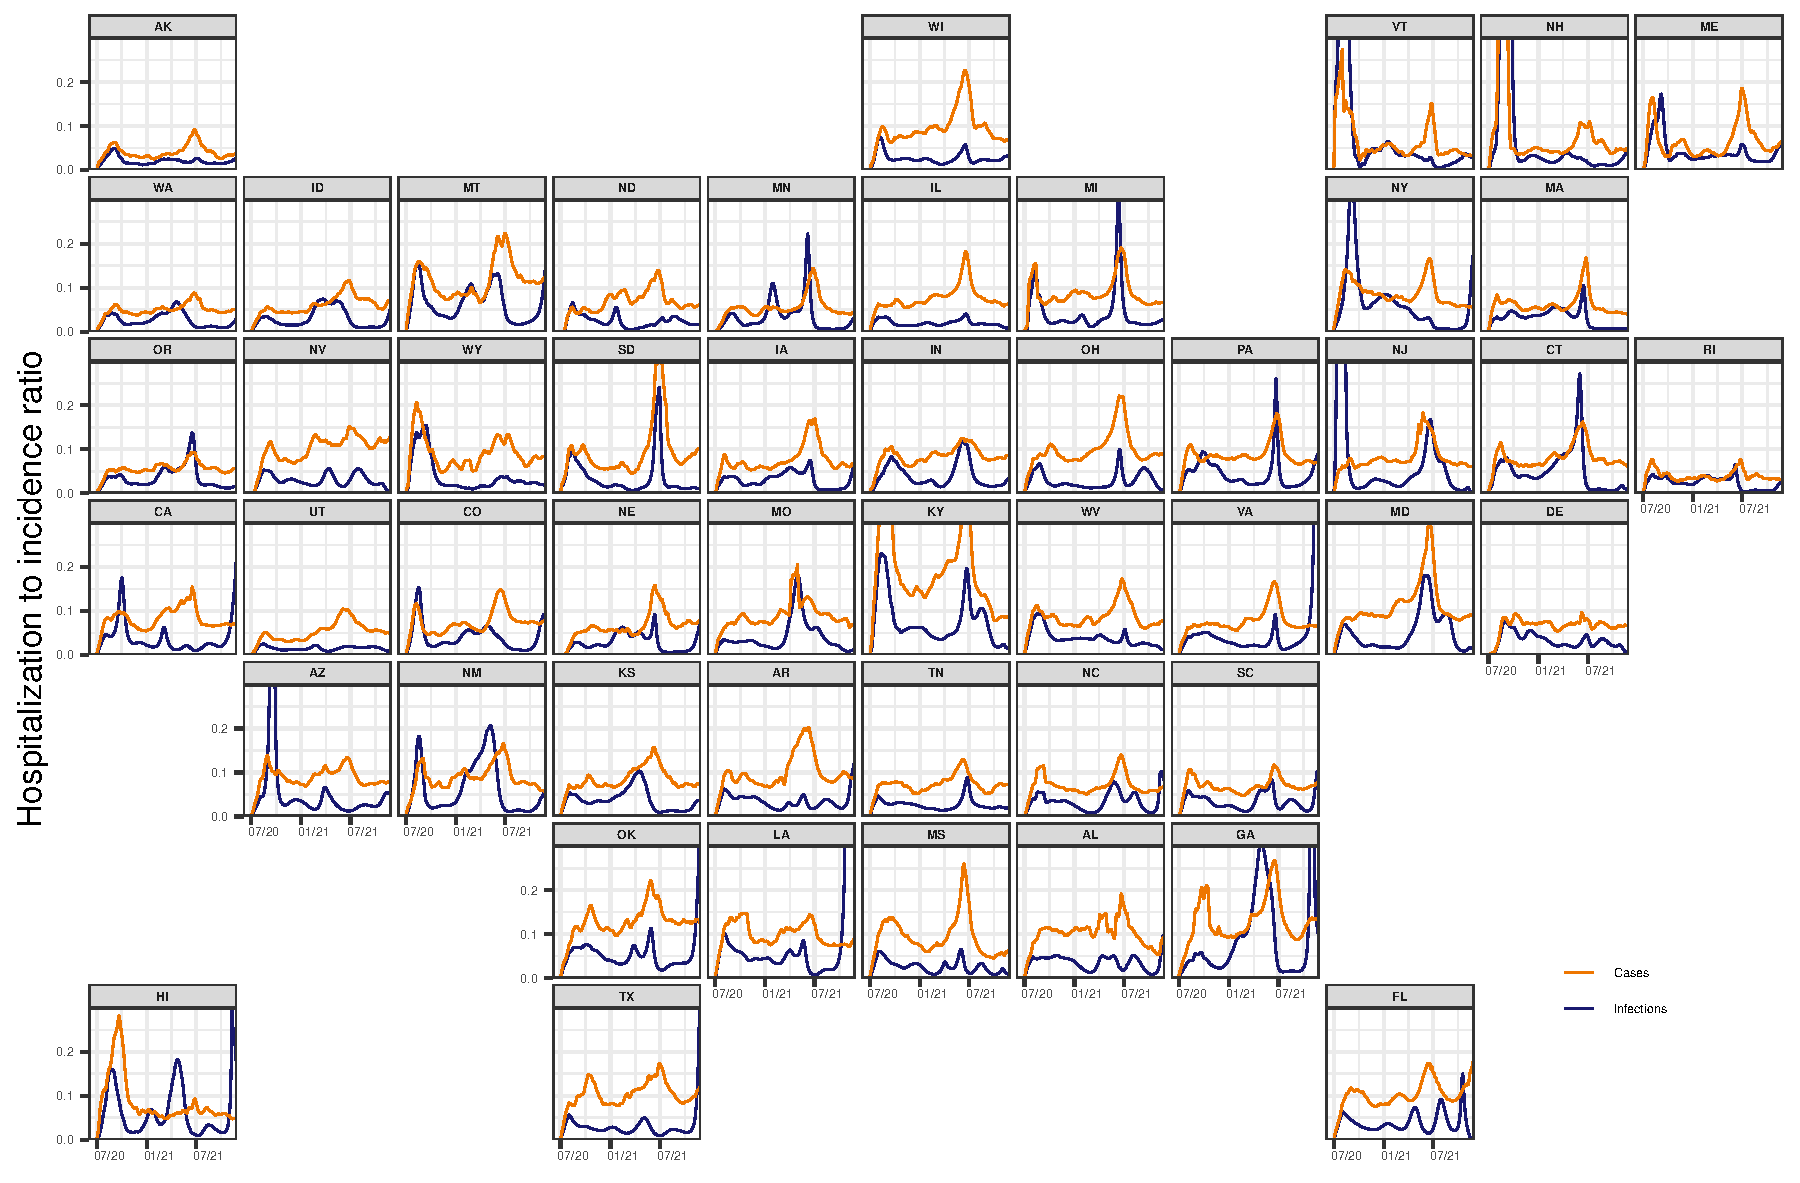
\includegraphics[width=\linewidth]{ihrs-1.pdf}
\caption{Time-varying IHR and CHR estimates for each state from June 1, 2020
to November 29, 2021, obtained using the corresponding optimal lag from the
systematic lag analysis. Note that the infection, case, and hospitalization
counts are subject to a center-aligned 7-day average to remove spurious day
of the week effects. Also note that the different starting points across
states are due to the availability of the hospitalization data.}
\label{fig:IHR_7dav}
\end{figure}
    

For each state, the CHRs tend to be larger in comparison to the IHRs. 
This is consistent with the claim that reported infections 
are more likely to require hospitalization than unreported infections. 
%For some states, the difference tends to be most pronounced during a major spike. Take, 
%for example, the major spike in mid-2021 in Mississippi, Arkansas, Wisconsin, Illinois, Ohio, or Maine. 

Both IHRs and CHRs exhibit similar
geospatial and temporal trends as those noted for infections. Namely,
states that are proximate (for example, North and South Carolina) tend
to exhibit similar temporal patterns in IHRs and CHRs. In addition, similar spikes are evident 
across many states during waves of infections that are driven
by variants of concern. For example, some states exhibit a striking increase in
hospitalizations in mid-2021, which coincides with the rapid takeover of the
Delta variant \citep{hodcroft2021covariants}. This finding aligns with previous
studies that found an increased risk in hospitalization due to Delta
\citep{twohig2022hospital, nyberg2022comparative}. Interestingly, when the
Ancestral variant predominates in 2020, there is a spike in the IHRs that rivals
or sometimes even surpasses that which is observed in the time of Delta. This situation is
most readily observable in the Northeastern states of 
New York, New Jersey, Vermont, and New Hampshire as well
as in some Western states such as Arizona, New Mexico, and Wyoming.

Overall, the relationship between infections and hospitalizations is
complicated. We observe intermittent spikes that punctuate longer periods where
the IHRs are relatively stabile, remaining below 0.1 hospitalizations per
infection. While we computed the IHRs and CHRs for all states, it is
important to note that both likely vary within states and depend on confounding
variables such as age and the presence of major comorbidities
\citep{russell2023comorbidities}. Therefore, it would be beneficial to account
for such variables in their calculations by, for example, stratifying infections
and hospitalizations by age to produce age-specific estimates of the IHRs for
each state~\citep{fox2023disproportionate}.





